\documentclass[12pt]{article}

\usepackage{sbc-template}

\usepackage{graphicx,url}
\usepackage{float}
\usepackage{verbatim}
\usepackage[english]{babel}

\sloppy

\title{Equirectangular Image Quality Assessment Tool Integrated into the Unity Editor}

\author{Adriano M. Gil\inst{1}, Thiago S. Figueira\inst{1}}

\address{Samsung Instituto de Desenvolvimento para a Informática da Amazônia
  (SIDIA)\\
  Manaus -- AM -- Brazil
  \email{\{adriano.gil,t.figueira\}@samsung.com}
}

\begin{document}

\maketitle

360 degrees pictures capture the surroundings of the user thus simulating the entire information available from a single point. 360 cameras such as the Samsung Gear 360 capture panoramic photos and store it in a suitable format for 360 visualization. Amongst the several possible formats for 360 degrees pictures, the equirectangular one is the most widely adopted. Virtual reality applications provide an immersive experience when using 360 media and give users the feeling of being inside the 360 picture as the virtual world simulates the one captured in the picture.

Virtual reality (VR) devices render the virtual world with a different image for each eye in order to emulate depth and as a result increase the feeling of presence within the context of the application. The technology behind VR headsets' displays have evolved, but they still face the challenge of offering a high density of pixels per field of view (FoV) degree. According to \cite{va1965visual}, the human eye has an estimated resolution of 60 pixels per degree which means that an average 100-degrees device should render its content at 6k resolution to provide the most realistic spacial emulation.

A 360 image viewer usually renders its contents in a sphere to mimic the natural placement of visual elements as they would be perceived by the user in the real world. A large amount of pixels is required to keep the quality of the pictures though. The research for the best possible visual quality means picking one in a given set of different exhibition formats each one with different distortion degrees along the existing 360 degrees. In order to decide the appropriate format and resolution for a 360 image it is necessary to take into consideration the device in which this picture will be displayed hence the necessity of a tool that is able to simulate devices and compare image settings so it provides the most suitable choice.

There are two approaches for image quality assessment: Subjective  and Objective metrics. The first one uses observers to evaluate and score a sequence of pictures and the second one makes automatic evaluations through mathematical models. In the context of tools, \textit{Unity Editor} is a game development engine for computers, mobile, console, virtual and augmented reality. It is both used by small development groups as well as big corporations such as Microsoft and Dinsey, it is also the most used development tool for virtual reality.

In this paper, we developed an equirectangular image quality assessment tool with objective metrics integrated into the Unity Editor. To make evaluations close to real case scenarios, our tool is capable of simulating visualization under predetermined field of view and resolution values. The image \ref{fig:tool} below presents the Unity Editor interface we built. 

\begin{figure}
    \centering
    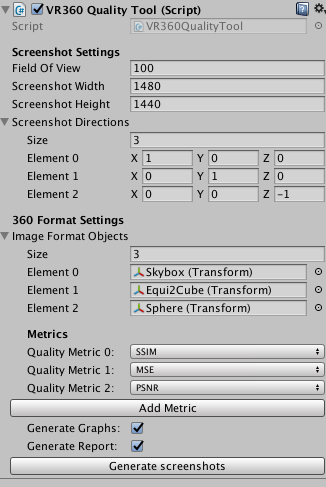
\includegraphics{images/tool.png}
    \caption{Our tool as seen directly on the Unity Editor}
    \label{fig:tool}
\end{figure}

The architecture of our implementation involves a C\# configuration layer in \textit{unity} and a \textit{python} layer for calculating the objective metrics for each of the Unity-generated images. Cross-tiered communication takes place through the creation of new processes within the Unity editor. Figure \ref{fig:toolarch} shows how the components are connected in our architecture.

\begin{figure}[ht]
\centering
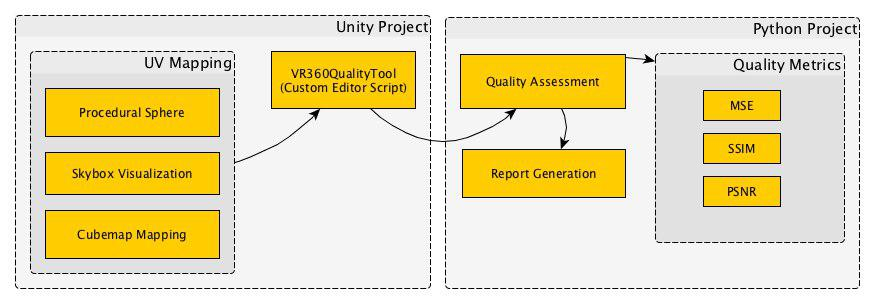
\includegraphics[width=\textwidth]{images/tool_arch_en.jpg}
\caption{The architecture of our implementation.}
\label{fig:toolarch}
\end{figure}

For a friendlier use, an editor interface has been developed in the form of a custom \textit{unity inspector}, that is, a custom view of our component in C\#. In this component you can define the angle of the field of view, define width and height as well as directions of the screenshots to be generated, define the comparison metrics to be used, and define whether graphs or a report will be generated at the end of the process.

The \textit{python} layer is responsible for evaluating the pairs of images generated by \textit{unity}. Using the \textit{scikit}, \textit{numpy}, and \textit{matplotlib} libraries, the images are evaluated and the result of each metric is saved in a report at the end, summarizing all results. 

With regards to the metrics, the goal of the objective evaluation is to develop a quantitative measure that can determine the quality of any given image. It is difficult, though, to find a single, objective, easy-to-calculate measurement that matches the visual inspection and is suitable for a variety of application requirements. As to address this problem, we are using three different metrics described below.

MSE or "Mean Square Error". The equation \ref{eq:mse} as follows:

\begin{equation}
MSE=\frac{1}{MN}\sum_{m=0}^{M-1}{\sum_{n=0}^{N-1}{e(m,n)^2}}
\label{eq:mse}
\end{equation}

SSIM is described by \cite{wang2004image} and can be calculated by the equation \ref{eq:ssim}.

\begin{equation}
SSIM(x,y)=\frac{(2*\mu_x*\mu_y+C_1)*(2*\sigma_{xy}+C_2)}{(\mu^2_x+\mu^2_y+C_1)*(\sigma^2_x+\sigma^2_y+C_2)}
\label{eq:ssim}
\end{equation}

Peak Signal-to-noise ratio (PSNR) is the most used metric for image quality assessment, the equation \ref{eq:psnr} is shown below:

\begin{equation}
PSNR = 10*log_{10}{\frac{(2^n-1)^2}{MSE}}
\label{eq:psnr}
\end{equation}

We used \textit{unity 2017.3.1 F} and \textit{python 2.7} to implement the proposed tool. The tool can be imported into any \textit{unity} project through a \textit{unitypackage}, a standard format from \textit{unity} to distribute resources and tools. To perform the quality assessment the button "Generate screenshots" is pressed and the value for each metric is calculated using the first image format as the default to evaluate the others. In figure \ref{fig:tool}, the reference image is the screenshot of the \textit{skybox}, which are compared with those obtained with the \textit{cubemap} and the spherical mapping. The results are summarized in the generated report, as demonstrated by the table below.

\begin{tabular}{l*{3}{c}r}
Metrics               & MSE & SSIM & PSNR \\
\hline
Direction 0 - Cubemap & 176,22 & 0,93 & 25,67 \\
Direction 1 - Cubemap & 125,63 & 0,93 & 27,14 \\
Direction 2 - Cubemap & 13,83 & 0,97 & 36,72 \\
Direction 0 - Sphere  & 88,56 & 0,88 & 28,66 \\
Direction 1 - Sphere  & 242,47 & 0,76 & 24,28 \\
Direction 2 - Sphere  & 96,26 & 0,86 & 28,30 \\
\label{tab:metrics_results}
\end{tabular}

Based on the obtained results, we found that the \textit{cubemap} pictures had better evaluation despite having an interpolation error. Such a mapping error can be corrected by using a \textit{fragment shader}. 

One of the disadvantages of our tool is that the user needs to know the metrics to be able to make the best parameters choice. For future work, we plan to use the current metrics to achieve a single and final evaluation value that should indicate the best result in an automated manner. Another improvement point identified is that the accuracy of the end result should be greater if the visualization is obtained directly from rendering on the mobile devices where VR applications can be executed. Thus, we also plan an embedded component in the application that allows you to reap results while running the application on the mobile device.

\bibliographystyle{sbc}
\bibliography{sbc-template}

\end{document}